\documentclass[11pt,a4paper]{article}
\usepackage[utf8]{inputenc}
\usepackage[T1]{fontenc}
\usepackage{amsmath,amssymb,amsfonts}
\usepackage{graphicx}
\usepackage{booktabs}
\usepackage{hyperref}
\usepackage{xcolor}
\usepackage{geometry}
\usepackage{fancyhdr}
\usepackage{enumitem}
\usepackage{tcolorbox}
\usepackage{tikz}
\usepackage{float}

\usetikzlibrary{shapes.geometric, arrows.meta, positioning}

\geometry{margin=2.5cm}
\hypersetup{colorlinks=true,linkcolor=blue,urlcolor=blue}
\graphicspath{{./models/}}

\pagestyle{fancy}
\fancyhf{}
\fancyhead[L]{Telco Customer Churn Prediction}
\fancyhead[R]{Technical Report}
\fancyfoot[C]{\thepage}

\title{\textbf{Telco Customer Churn Prediction}\\[0.5cm]
\large A Complete Machine Learning Pipeline}
\author{Machine Learning Project Report}
\date{January 2026}

\begin{document}

\maketitle

\begin{abstract}
This report presents a complete machine learning solution for predicting customer churn in the telecommunications industry. We walk through every step from data exploration to model deployment, making it easy for readers to understand and replicate. The project includes four machine learning models, a REST API, and a web interface. Key finding: tenure (customer lifespan) and contract type are the strongest predictors of churn.
\end{abstract}

\tableofcontents
\newpage

%==============================================================================
\section{Introduction}
%==============================================================================

\subsection{What is Customer Churn?}
\textbf{Customer churn} happens when a customer stops using a company's services. In the telecom industry, this means a customer cancels their phone or internet subscription and moves to a competitor.

\textbf{Why does it matter?}
\begin{itemize}
    \item Getting a new customer costs 5-7 times more than keeping an existing one
    \item A 5\% increase in customer retention can boost profits by 25-95\%
    \item Early prediction allows companies to offer incentives before customers leave
\end{itemize}

\subsection{Our Goal}
We want to build a machine learning model that can predict which customers are likely to leave. This is a \textbf{binary classification} problem:
\begin{itemize}
    \item \textbf{Input:} Customer information (demographics, services, billing)
    \item \textbf{Output:} Will this customer churn? (Yes or No)
\end{itemize}

\subsection{Dataset Used}
We used the \textbf{IBM Telco Customer Churn} dataset with:
\begin{itemize}
    \item 7,043 customers
    \item 21 features per customer
    \item 26.5\% of customers actually churned (left the company)
\end{itemize}

%==============================================================================
\section{Exploring the Data (EDA)}
%==============================================================================

\subsection{Understanding the Target Variable}
Our target variable is \textbf{Churn} with two values:
\begin{itemize}
    \item \textbf{No} (stayed): 5,174 customers (73.5\%)
    \item \textbf{Yes} (left): 1,869 customers (26.5\%)
\end{itemize}

\begin{figure}[H]
\centering
\includegraphics[width=0.85\textwidth]{churn_distribution.png}
\caption{The data is imbalanced---most customers stayed. This is typical in real-world churn scenarios.}
\end{figure}

\textbf{Important note:} Because only 26.5\% of customers churned, a model that always predicts "No churn" would be 73.5\% accurate but completely useless! This is why we use metrics like F1-Score and Recall instead of just Accuracy.

\subsection{What Makes Customers Leave?}
We analyzed various factors to understand what drives churn:

\begin{figure}[H]
\centering
\includegraphics[width=0.95\textwidth]{churn_by_categories.png}
\caption{Churn rates vary significantly across different customer segments.}
\end{figure}

\textbf{Key discoveries:}
\begin{enumerate}
    \item \textbf{Contract type matters most:}
    \begin{itemize}
        \item Month-to-month contracts: 43\% churn rate (very high!)
        \item One-year contracts: 11\% churn rate
        \item Two-year contracts: only 3\% churn rate
    \end{itemize}
    
    \item \textbf{Payment method affects churn:}
    \begin{itemize}
        \item Electronic check: 45\% churn (highest!)
        \item Automatic payments: around 15\% churn
    \end{itemize}
    
    \item \textbf{New customers are at highest risk:}
    \begin{itemize}
        \item Customers in their first year: 47\% churn
        \item Customers with 6+ years: only 7\% churn
    \end{itemize}
\end{enumerate}

\subsection{Numeric Features Analysis}

\begin{figure}[H]
\centering
\includegraphics[width=0.9\textwidth]{numeric_by_churn.png}
\caption{Comparing numeric features between customers who stayed vs. left.}
\end{figure}

\textbf{What we learned:}
\begin{itemize}
    \item Churners have \textbf{shorter tenure} (fewer months with the company)
    \item Churners pay \textbf{higher monthly charges} on average
    \item Churners have \textbf{lower total charges} (because they left early)
\end{itemize}

%==============================================================================
\section{The Machine Learning Pipeline}
%==============================================================================

Below is our complete pipeline showing how data flows from raw input to final prediction:

\begin{figure}[H]
\centering
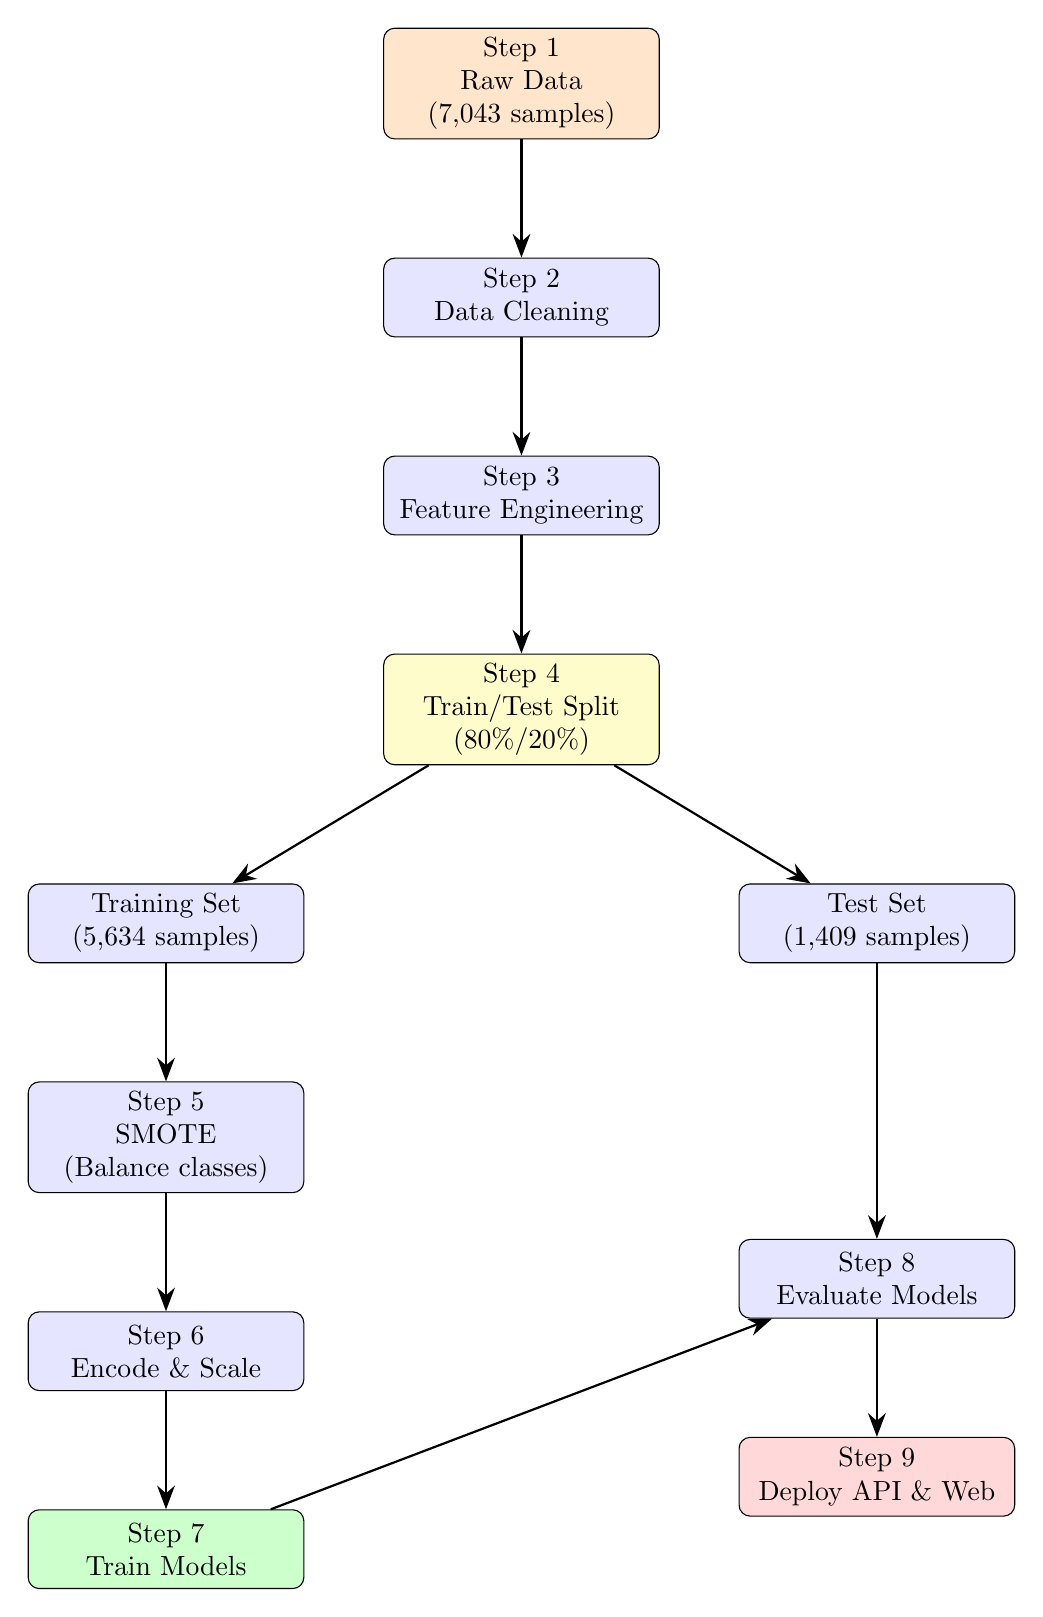
\begin{tikzpicture}[
    node distance=1.5cm,
    box/.style={rectangle, draw, fill=blue!10, minimum width=3.5cm, minimum height=1cm, align=center, rounded corners},
    arrow/.style={-{Stealth[length=3mm]}, thick}
]

% Main flow - vertical left side
\node[box, fill=orange!20] (raw) {Step 1\\Raw Data\\(7,043 samples)};
\node[box, below=of raw] (clean) {Step 2\\Data Cleaning};
\node[box, below=of clean] (feature) {Step 3\\Feature Engineering};
\node[box, below=of feature, fill=yellow!20] (split) {Step 4\\Train/Test Split\\(80\%/20\%)};

% Branch - training path
\node[box, below left=1.5cm and 1cm of split] (train) {Training Set\\(5,634 samples)};
\node[box, below=of train] (smote) {Step 5\\SMOTE\\(Balance classes)};
\node[box, below=of smote] (encode) {Step 6\\Encode \& Scale};
\node[box, below=of encode, fill=green!20] (model) {Step 7\\Train Models};

% Branch - testing path
\node[box, below right=1.5cm and 1cm of split] (test) {Test Set\\(1,409 samples)};
\node[box, below=3.5cm of test] (eval) {Step 8\\Evaluate Models};

% Final
\node[box, below=1.5cm of eval, fill=red!15] (deploy) {Step 9\\Deploy API \& Web};

% Arrows
\draw[arrow] (raw) -- (clean);
\draw[arrow] (clean) -- (feature);
\draw[arrow] (feature) -- (split);
\draw[arrow] (split) -- (train);
\draw[arrow] (split) -- (test);
\draw[arrow] (train) -- (smote);
\draw[arrow] (smote) -- (encode);
\draw[arrow] (encode) -- (model);
\draw[arrow] (model) -- (eval);
\draw[arrow] (test) -- (eval);
\draw[arrow] (eval) -- (deploy);

\end{tikzpicture}
\caption{Our machine learning pipeline has 9 main steps. Notice that SMOTE is only applied to training data, not test data.}
\end{figure}

\subsection{Step 1-2: Data Cleaning}
\textbf{Problem found:} The TotalCharges column had 11 empty values (new customers who haven't been charged yet).

\textbf{Solution:} We filled these with 0, which makes sense because new customers have zero charges.

\subsection{Step 3: Feature Engineering}
We created two new features to help our model:

\textbf{Feature 1: Tenure Group}

Instead of using the exact number of months, we grouped customers by their tenure phase:

\begin{table}[H]
\centering
\begin{tabular}{lcc}
\toprule
\textbf{Group} & \textbf{Tenure} & \textbf{Churn Rate} \\
\midrule
New Customer & 0-12 months & 47\% (highest!) \\
Growing & 12-24 months & 28\% \\
Established & 24-48 months & 19\% \\
Loyal & 48-72 months & 13\% \\
Very Loyal & 72+ months & 7\% (lowest) \\
\bottomrule
\end{tabular}
\caption{Customers follow a predictable loyalty pattern.}
\end{table}

\textbf{Feature 2: Number of Services}

We counted how many additional services each customer uses (security, backup, streaming, etc.). More services = more "locked in" = less likely to leave.

\begin{figure}[H]
\centering
\includegraphics[width=0.9\textwidth]{engineered_features.png}
\caption{Both new features show clear patterns related to churn.}
\end{figure}

\subsection{Step 4: Train/Test Split}
We split the data into two parts:
\begin{itemize}
    \item \textbf{Training set (80\%):} 5,634 customers for teaching the model
    \item \textbf{Test set (20\%):} 1,409 customers for honest evaluation
\end{itemize}

\begin{tcolorbox}[colback=red!5!white,colframe=red!75!black,title=Critical Rule]
We split the data \textbf{before} applying SMOTE. If we SMOTE first, fake data can leak into the test set and give us inflated (wrong) results!
\end{tcolorbox}

\subsection{Step 5: SMOTE (Handling Class Imbalance)}
\textbf{Problem:} Only 26.5\% of training data are churners. The model might ignore them.

\textbf{Solution:} SMOTE creates synthetic (artificial) examples of churners to balance the classes.

\textbf{How SMOTE works:}
\begin{enumerate}
    \item Pick a churning customer
    \item Find their nearest neighbors (similar churners)
    \item Create new points between them
\end{enumerate}

Mathematically: $x_{new} = x_i + \lambda \times (x_j - x_i)$ where $\lambda$ is random between 0 and 1.

\textbf{Result:} Training set goes from 1,495 to 4,139 churners (now balanced 50:50).

\subsection{Step 6: Encoding and Scaling}

\textbf{Encoding:} Convert text to numbers so the model can understand.
\begin{itemize}
    \item \textbf{Binary features} (Male/Female, Yes/No): Convert to 0/1
    \item \textbf{Multi-category features} (Contract type): Create separate 0/1 columns for each option
\end{itemize}

\textbf{Scaling:} Normalize numbers to similar ranges using the z-score formula:
$$z = \frac{x - \mu}{\sigma}$$
This makes features with large values (like TotalCharges) comparable to small ones (like tenure).

%==============================================================================
\section{Evaluation Metrics Explained}
%==============================================================================

For churn prediction, we use several metrics from the confusion matrix:

\begin{table}[H]
\centering
\begin{tabular}{c|cc}
& \textbf{Predicted: Stay} & \textbf{Predicted: Leave} \\
\hline
\textbf{Actually Stayed} & True Negative (TN) & False Positive (FP) \\
\textbf{Actually Left} & False Negative (FN) & True Positive (TP) \\
\end{tabular}
\caption{Confusion Matrix Layout}
\end{table}

\textbf{Key Formulas:}

\begin{align}
\text{Accuracy} &= \frac{TP + TN}{\text{Total}} \quad \text{(Overall correctness---misleading for imbalanced data!)}\\[8pt]
\text{Precision} &= \frac{TP}{TP + FP} \quad \text{(Of those we flagged, how many were right?)}\\[8pt]
\text{Recall} &= \frac{TP}{TP + FN} \quad \text{(Of actual churners, how many did we catch?)}\\[8pt]
\text{F1-Score} &= 2 \times \frac{\text{Precision} \times \text{Recall}}{\text{Precision} + \text{Recall}} \quad \text{(Balance of both)}
\end{align}

\textbf{For churn prediction, Recall is most important} because missing a churner (False Negative) means losing a customer forever.

%==============================================================================
\section{Model Training and Results}
%==============================================================================

\subsection{Models We Tested}
\begin{enumerate}
    \item \textbf{Logistic Regression:} Simple, interpretable baseline
    \item \textbf{Random Forest:} Ensemble of 100 decision trees
    \item \textbf{XGBoost:} Advanced gradient boosting algorithm
    \item \textbf{Neural Network:} Deep learning with 2 hidden layers (16 and 8 neurons)
\end{enumerate}

\subsection{Results Comparison}

\begin{table}[H]
\centering
\caption{Model Performance on Test Set (Honest Evaluation)}
\begin{tabular}{lccccc}
\toprule
\textbf{Model} & \textbf{Accuracy} & \textbf{Precision} & \textbf{Recall} & \textbf{F1-Score} & \textbf{AUC} \\
\midrule
Neural Network & 77.9\% & 56.8\% & 69.0\% & \textbf{62.3\%} & 84.1\% \\
Logistic Regression & 74.3\% & 51.0\% & \textbf{80.0\%} & 62.3\% & 84.1\% \\
Random Forest & 76.8\% & 55.2\% & 66.8\% & 60.5\% & 84.0\% \\
XGBoost & 78.1\% & 58.5\% & 60.7\% & 59.6\% & 83.4\% \\
\bottomrule
\end{tabular}
\end{table}

\begin{figure}[H]
\centering
\includegraphics[width=0.95\textwidth]{model_comparison.png}
\caption{Left: Metrics comparison. Right: ROC curves showing all models have similar discriminative ability.}
\end{figure}

\subsection{Confusion Matrices}

\begin{figure}[H]
\centering
\includegraphics[width=0.8\textwidth]{confusion_matrices.png}
\caption{Confusion matrices for all four models.}
\end{figure}

\subsection{Which Model is Best?}
\begin{itemize}
    \item \textbf{Best F1-Score:} Neural Network (62.3\%)
    \item \textbf{Best Recall:} Logistic Regression (80\%)---catches 80\% of churners!
    \item \textbf{Best Precision:} XGBoost (58.5\%)---fewest false alarms
\end{itemize}

\textbf{Recommendation:} Use Logistic Regression if you want to catch as many churners as possible, even at the cost of some false alarms.

\subsection{What Features Matter Most?}

\begin{figure}[H]
\centering
\includegraphics[width=0.8\textwidth]{feature_importance.png}
\caption{Top features according to Random Forest.}
\end{figure}

The most important predictors of churn are:
\begin{enumerate}
    \item Total charges and monthly charges
    \item Tenure (how long they've been a customer)
    \item Contract type
    \item Number of services
\end{enumerate}

%==============================================================================
\section{Deployment}
%==============================================================================

\subsection{System Architecture}
The deployment consists of two main components:
\begin{enumerate}
    \item \textbf{Backend (FastAPI):} REST API that loads all trained models and handles predictions
    \item \textbf{Frontend (Streamlit):} Interactive web interface for users to input customer data
\end{enumerate}

\subsection{REST API (FastAPI)}
We created a web service that accepts customer data and returns predictions.

\textbf{Key Features:}
\begin{itemize}
    \item Loads all 4 models on startup (Neural Network, Logistic Regression, Random Forest, XGBoost)
    \item Supports \textbf{model selection}---users can choose which model to use
    \item Automatic feature engineering (Tenure\_Group, Number\_of\_Services)
    \item Automatic label encoding for binary columns
    \item Risk level classification (Low/Medium/High) with recommendations
\end{itemize}

\textbf{API Endpoints:}
\begin{table}[H]
\centering
\begin{tabular}{llp{6cm}}
\toprule
\textbf{Method} & \textbf{Endpoint} & \textbf{Description} \\
\midrule
GET & \texttt{/} & API information and links \\
GET & \texttt{/health} & Health check, lists loaded models \\
POST & \texttt{/predict} & Make prediction with selected model \\
GET & \texttt{/model-info} & Get model details \\
\bottomrule
\end{tabular}
\end{table}

\textbf{How to run:}
\begin{enumerate}
    \item Open terminal in project folder
    \item Activate environment: \texttt{.\textbackslash venv\textbackslash Scripts\textbackslash activate}
    \item Start server: \texttt{uvicorn app.api:app --reload --port 8000}
    \item Open browser: \texttt{http://localhost:8000/docs}
\end{enumerate}

\subsection{Web Interface (Streamlit)}
For non-technical users, we built an interactive web app with rich features.

\textbf{Key Features:}
\begin{itemize}
    \item \textbf{Model Selection:} Dropdown in sidebar to choose between 4 models
    \item \textbf{Interactive Inputs:} Sliders, radio buttons, and dropdowns for all customer fields
    \item \textbf{Color-coded Results:} Green (Low risk), Yellow (Medium risk), Red (High risk)
    \item \textbf{Business Recommendations:} Actionable advice based on risk level
    \item \textbf{Customer Profile Summary:} Expandable section showing all input data
\end{itemize}

\textbf{User Interface Layout:}
\begin{itemize}
    \item \textbf{Sidebar:} Model selection dropdown and about information
    \item \textbf{Column 1 (Demographics):} Gender, Senior Citizen, Partner, Dependents
    \item \textbf{Column 2 (Services):} Phone, Internet, Security, Streaming options
    \item \textbf{Column 3 (Account):} Tenure, Contract, Billing, Payment, Charges
    \item \textbf{Results Area:} Prediction, Probability, Risk Level, Recommendations
\end{itemize}

\textbf{How to run:}
\begin{enumerate}
    \item Start the API first (see above)
    \item In a new terminal, run: \texttt{streamlit run app/streamlit\_app.py}
    \item Open browser: \texttt{http://localhost:8501}
\end{enumerate}

\subsection{Preprocessing in Deployment}
When making predictions in production, the API performs these preprocessing steps automatically:

\begin{enumerate}
    \item \textbf{Feature Engineering:}
    \begin{itemize}
        \item Computes Tenure\_Group from tenure value
        \item Computes Number\_of\_Services by counting "Yes" values
    \end{itemize}
    
    \item \textbf{Label Encoding:} Converts binary columns to 0/1:
    \begin{itemize}
        \item gender: Female$\rightarrow$0, Male$\rightarrow$1
        \item Partner, Dependents, PhoneService, PaperlessBilling: No$\rightarrow$0, Yes$\rightarrow$1
    \end{itemize}
    
    \item \textbf{Preprocessing Pipeline:} Applies saved ColumnTransformer (scaling and one-hot encoding)
    
    \item \textbf{Prediction:} Uses selected model to predict probability
\end{enumerate}

%==============================================================================
\section{Lessons Learned: Data Leakage}
%==============================================================================

\textbf{What went wrong initially:}

We accidentally applied SMOTE before splitting the data. This caused synthetic (fake) churners to appear in our test set.

\textbf{The evidence:}
\begin{itemize}
    \item Expected test set churn rate: 27\% (natural)
    \item Actual test set churn rate: 50\% (artificial!)
\end{itemize}

\textbf{Impact:}
\begin{itemize}
    \item Before fix: F1-Score = 85\% (fake, too good to be true)
    \item After fix: F1-Score = 62\% (honest, realistic)
\end{itemize}

\textbf{Lesson:} Always split data before any data augmentation!

%==============================================================================
\section{Business Recommendations}
%==============================================================================

Based on our analysis, here are actionable recommendations:

\begin{table}[H]
\centering
\begin{tabular}{p{4cm}p{3cm}p{6cm}}
\toprule
\textbf{Risk Factor} & \textbf{Churn Rate} & \textbf{Recommended Action} \\
\midrule
Month-to-month contract & 43\% & Offer discounts for 1-year upgrade \\
New customer (0-12 months) & 47\% & Special onboarding program \\
Electronic check payment & 45\% & Incentive for auto-pay enrollment \\
Few services subscribed & 35\% & Bundle package promotions \\
Fiber optic internet & 42\% & Check service quality issues \\
\bottomrule
\end{tabular}
\caption{Targeted retention strategies for high-risk segments.}
\end{table}

%==============================================================================
\section{Conclusion}
%==============================================================================

\subsection{What We Achieved}
\begin{enumerate}
    \item Built a complete ML pipeline from data to deployment
    \item Trained 4 models including deep learning
    \item Identified and fixed a critical data leakage issue
    \item Created API and web interface for real-world use
\end{enumerate}

\subsection{Future Improvements}
\begin{enumerate}
    \item \textbf{Lower the prediction threshold} to catch more churners
    \item \textbf{Tune hyperparameters} for better performance
    \item \textbf{Add model explainability} using SHAP values
    \item \textbf{Monitor performance} over time for drift
\end{enumerate}

\end{document}
